\documentclass[a4paper,twoside,openany,notitlepage]{book}
\usepackage[T1]{fontenc}
\usepackage[utf8]{inputenc}
\usepackage[english,italian]{babel}
\usepackage{geometry}
\geometry{a4paper,top=3cm,bottom=3cm,left=2.5cm,right=2.5cm,%
	heightrounded,bindingoffset=5mm}
\usepackage{amsmath}
\usepackage{amssymb}
\usepackage{amsthm}
\usepackage{booktabs}
\usepackage{caption} %per inserire descrizione immagini
%\usepackage{sidecap} %per inserire descrizioni laterali alle immagini
\usepackage{wrapfig} %per inserire immagini a lato pagina, wrappando il testo intorno
\usepackage{graphicx} %impaginazione
\usepackage{blindtext} %boh
\usepackage{isotope} %scrittura isotopi
\usepackage{url} %scrittura di link
\usepackage{hyperref} %collegamenti ipertestuali e link web

%Per l'inserimento immagini la guida molto utile di wikipedia:
%https://en.wikibooks.org/wiki/LaTeX/Floats,_Figures_and_Captions

%Settaggio comandi grafici
%\renewcommand{\caption*}[1]{\begin{center}{\caption*{#1}}}%inserimento testo centrato sotto immagini
\captionsetup{justification=centering}

%Definizione comando email e settaggio del pacchetto hyperref
\newcommand{\mail}[1]{\href{mailto:#1}{\nolinkurl{#1}}}
\hypersetup{hidelinks}

%Definizione comando per notazione vettoriale e simbolo definizione
\renewcommand{\vec}{\boldsymbol}
\newcommand{\Def}{\overset{\mathit{def}}{=}}

%Definizione comando per notazione scientifica
\newcommand{\e}[1]{\cdot 10^{#1}}

%Definizione unità di misura
\newcommand{\angstrom}{\mbox{\normalfont\AA}}

%Funzioni trigonometriche iperboliche ed inverse
\DeclareMathOperator{\sech}{sech}
\DeclareMathOperator{\csch}{csch}
\DeclareMathOperator{\arcsec}{arcsec}
\DeclareMathOperator{\arccot}{arcCot}
\DeclareMathOperator{\arccsc}{arcCsc}
\DeclareMathOperator{\arccosh}{arcCosh}
\DeclareMathOperator{\arcsinh}{arcsinh}
\DeclareMathOperator{\arctanh}{arctanh}
\DeclareMathOperator{\arcsech}{arcsech}
\DeclareMathOperator{\arccsch}{arcCsch}
\DeclareMathOperator{\arccoth}{arcCoth}

%Definizione comandi per teoremi, enunciati ecc
\theoremstyle{definition}
\newtheorem{definizione}{Definizione}
\newtheorem*{definizionenn}{Definizione}
\newtheorem*{principio}{Principio}
\newtheorem*{postulato}{Postulato}
\newtheorem*{exmp}{Esempio}
\newtheorem{exrc}{Esercizio}
\newtheorem{sol}{Soluzione}

\theoremstyle{plain}
\newtheorem{teorema}{Teorema}
\newtheorem*{teoremann}{Teorema}
\newtheorem*{lemma}{Lemma}
\newtheorem*{proprietà}{Si trova che}

\begin{document}
\frontmatter
\author{Volpe Francesco}
\title{Appunti di Astrofisica sperimentale}
%\mail{francesco.volpe1998@gmail.com}
\date{}
\maketitle

\pagestyle{plain}
\tableofcontents

\chapter*{Prefazione}

Il corso di cui si riportano gli appunti è dell'anno accademico 2020/2021 presso l'università di Ferrara ed è suddiviso in tre parti: la prima tenuta dal professore P. Rosati, la seconda tenuta dal professore C. Guidorzi, la terza (prettamente sperimentale) tenuta dal prof E. Virgilli.

I concetti di base del corso sono ripresi e integrati dal corso di Astrofisica del primo semestre del terzo anno, a cui si aggiungono alcuni dettagli sulle misurazioni fotometriche e una trattazione aggiuntiva sulla misurazione delle distanze. Sulle grandi distanze verranno introdotti anche alcuni concetti del corso opzionale di Cosmologia, poiché risulterà impossibile continuare una trattazione classica. Finita la prima parte di trattazione dei telescopi e di tecniche di misura basate sui raggi x e sui "soft" x si passa alla seconda parte del corso, che tratterà la misura di masse, i sistemi binari fino ad arrivare ad accennare alle stelle compatte e i buchi neri, parlerà inoltre di onde gravitazionali, dell'astronomia multi-messaggera (che verrà introdotta nella prima parte del corso) e di tecniche di rivelazione di nuovi pianeti extra-solari. La terza parte tratterà la fisica dei rivelatori e l'astrofisica ad alte energie (quindi oltre i raggi x), la spettroscopia e fondamenti di analisi di X e $\gamma$, con esperienze al LARIX (laboratorio interrato al polo scientifico-tecnologico a Ferrara) e se sarà possibile all'INAF a Bologna.

I libri principalmente usati sarano Astronomy Methods - H. Bradt, Astronomy principles and practice - A.E.Roy \& D. Clarke, Fundamental Astronomy - Kattunen.

\mainmatter

\input{Capitoli/Capitolo1.tex}

\input{Capitoli/Capitolo2.tex}

\chapter{Spettroscopia}

\section{Introduzione agli spettroscopi e alle quantità spettrali}

Un pilastro informativo in astrofisica è l'analisi dei profili spettrali, noto come \textbf{sprettroscopia}, in grado di dare molte informazioni riguardo le sorgenti, in quanto ogni profilo è tipico di un certo tipo di processo di emissione ed è quindi utile per capire la fisica che sta dietro i segnali che riceviamo. L'incipit di questa analisi sta innanzitutto in un processo di isolamento e collimazione della luce proveniente dalla specifica sorgente che si vuole studiare, tipicamente svolto dal telescopio, dopo di che il fascio viene fatto espandere tramite una fenditura, posta solitamente nel fuoco stesso del telescopio, per poi passare attraverso un \textit{elemento dispersivo}, come ad esempio un prisma. L'elemento dispersore rende possibile l'analisi dello spettro spacchettando il fascio in arrivo in tutte le lunghezze d'onda, per rendere questo possibile è necessario che il fascio incidente arrivi parallelo, poichè la rifrazione è in funzione sia della lunghezza che dell'angolo incidente.

\begin{figure}[h]
    \centering
    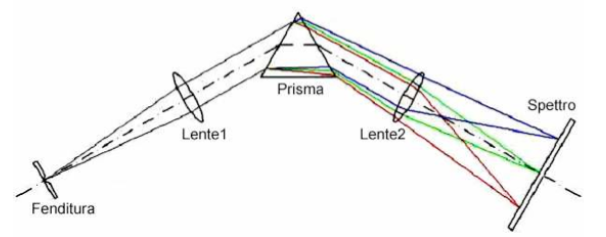
\includegraphics[width=0.55\textwidth]{Immagini/Capitolo3/Spettrografo_schema.PNG}
    \caption{Rappresentazione schematica di uno spettroscopio a prisma}
    \label{im:schema-spettroscopio-prisma}
\end{figure}

Per togliere quest'ultimo elemento e analizzare solo il percorso di rifrazione, si introducono delle lenti focalizzanti tra la fenditura e il prisma, ma anche tra il prisma e successivamente il piano focale, per cui il fascio incida da prima parallelamente, per poi essere reso ancora più separato a seguito della dispersione sul piano focale, in modo da rendere l'analisi più effettiva. Quanto descritto è schematizzato nell'immagine \ref{im:schema-spettroscopio-prisma}.

\begin{wrapfigure}{l}{0.3\textwidth}
    \centering
    \vspace{-10pt}
    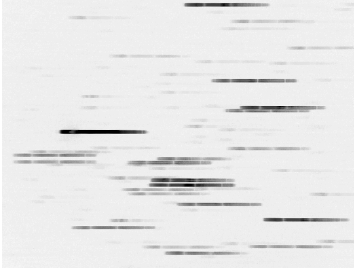
\includegraphics[width=0.29\textwidth]{Immagini/Capitolo3/Spettro_cielo_generico.PNG}
    \caption*{Spettro di una parte di cielo, dispersione orizzontale verso destra}
    \vspace{-15pt}
\end{wrapfigure}

I fasci uscenti, separati ulteriormente dal secondo specchio, andranno poi fuocheggiati da un secondo obiettivo, per fare ciò si regola il sistema ottico in modo da inviare lo spettro orientato lungo uno degli assi del CCD. Questa tecnica crea un'immagine a righe, le quali si estendono tutte in una direzione specifica, che è la \textit{direzione di dispersione}, come si vede in immagine, la quale è frutto di uno spettroscopio in cui si è osservato un pezzo di cielo, senza isolare una sorgente specifica, per cui ad ogni riga corrisponde una differente sorgente. Per passare ad una descrizione più formale, risulta necessario partire proprio dal concetto di \textit{dispersione angolare} $d\beta/d\lambda$, che consiste, come è facilmente intuibile, nella differenza di angolo di dispersione $d\beta$ rapportato alla differenza di lunghezza d'onda $d\lambda$ tra due onde adiacenti. A seguito della dispersione, le onde vengono poi focalizzate su un CCD, che una volta calibrato avrà la sua focale equivalente $f$. Ora, se i raggi arrivano paralleli opichè rifocalizzati, significa che ad ogni raggio disperso ad angolo $\beta$ corrisponderà una distanza diversa sul piano focale, chiamando $l$ la distanza dall'asse ottico e ricordando la correlazione diretta tra angolo di dispersione e distanza lineare sul piano focale, si ricava la dispersione lineare:
\begin{equation}
    \frac{dl}{d\lambda} = f \frac{d\beta}{d\lambda}
\end{equation}
Dove la dispersione angolare è quella propria dell'elemento dispersore dell'apparato. La misura finale dello shift lineare può essere sia in $mm/\angstrom$ che più comodamente in $pxl/\angstrom$, essendo i pixel quello con cui poi si va effettivamente a lavorare, un esempio della comodità di avere un'equazione espressa nelle seconde è avere un riferimento diretto a quanti pixel di differenza ci siano per una variazione $d\lambda$ di lunghezza d'onda.

\begin{wrapfigure}{r}{0.4\textwidth}
    \centering
    \vspace{-10pt}
    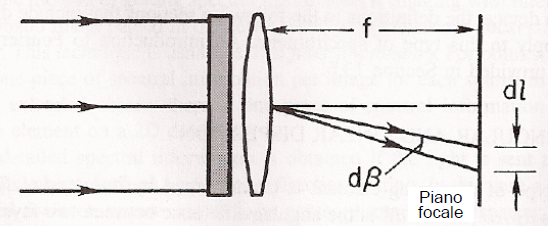
\includegraphics[width=0.39\textwidth]{Immagini/Capitolo3/Spettroscopia_schema_dispersione_lineare.PNG}
    \caption*{Schema dispersione lineare}
    \vspace{-10pt}
\end{wrapfigure}

Questa quantità viene spesso usata nel suo inverso, per motivi di pura comodità, ossia come $d\lambda/dl$, ovviamente con le unità invertite che siano $\angstrom/mm$ o $\angstrom/pxl$, in tal senso viene inteso come campionamento in pixel lungo la direzione di dispersione delle onde al variare della propria lunghezza d'onda. Così come è importante, nel caso visto di imaging, non confondere la risoluzione angolare di un sistema ottico con il suo campionamento, allo stesso modo in spettroscopia non va confusa la dispersione lineare di uno spettrografo con la sua risoluzione. Parlando di ciò, si definisce la \textbf{risoluzione spettrale} $R$ di uno spettrografo come la capacità di risolvere onde a lunghezza d'onda vicine, formalmente si definisce come:
\begin{equation}
    \label{def:risoluzione-spettrale}
    R = \frac{\lambda}{\Delta\lambda}
\end{equation}
Intesa come capacità di risolvere due onde di cui una a lunghezza d'onda $\lambda$ e l'altra a lunghezza d'onda $\lambda+\Delta\lambda$. Dando una classificazione rapida, si intendono a bassa risoluzione gli spettrografi con $R\sim 100-600$, a risoluzione intermedia con $R\sim 1000-500$, e ad alta risoluzione con $R\sim 10^4-10^5$. Da questa quantità si arriva a definire il \textbf{range spettrale} $1/R$ come l'inverso della risoluzione spettrale, per cui si ha $1/R \sim \Delta\lambda/\lambda$, corrispondente alla definizione di redshift. Introdotte queste quantità, ogni spettrografo ha la sua funzione, nel caso si vogliano studiare corpi di cui è ignoto il redshift converrà adottare una bassa risoluzione che permetterà così di avere un ampio range di analisi. Un caso diverso è quello in cui si vogliano misurare le microvariazioni di effetto Doppler di una stella derivate dal suo moto attorno al centro di massa, ad esempio qualora si sospetti ci sia un micropianeta in orbita attorno a lei e che crei un moto dell'ordine dei $m/s$ (quindi estremamente piccolo), per cui sarà necessaria una risoluzione molto alta per osservare dei piccolissimi shift nelle lunghezze d'onda, corrispodentia queste piccolissime variazioni di velocità. Ci saranno poi anche tutti i casi intermedi rispetto agli esempi presi, questa dualità tra range e risoluzione rimane comunque imprescindibile, ma bisogna anche tenere conto della dispersione. Di fatti il sistema ottico dello spettrografo deve essere calibrato in modo che ad una certa risoluzione, ad esempio di $1\, \angstrom$, corrispondano tre o quattro pixel di dispersione in modo che poi due lunghezze d'onda siano effettivamente risolvibili a quella risoluzione, speculare a quanto visto nel caso di imaging tra campionamento e risoluzione. La limitazione fondamentale per cui si fanno questo tipi di ragionamenti è il fatto che il sistema ottico ha dimensioni finite così come lo hanno i CCD che fungono da detector nelle strumentazioni moderne, nel caso non avessimo delle dimensioni limitanti si potrebbe studiare ad alta risoluzione aumentando costantemente il numero di CCD in dotazione, in modo si manterebbe anche un ampio spettro.

Nei telescopi moderni si preferisce adoperare dei \textit{reticoli di diffrazione} (reflection/diffraction gratings) come elemento dispersore al posto dei prismi, che altro non sono che superfici piane riflettenti cosparse di solchi lineari superficiali. Questi reticoli possono avere dimensioni ridotte sull'ordine dei cm nei telescopi minori, così come arrivare a dimensioni di mezzo metro o maggiori. Grazie ad essi, oltre ad aver raggiunto valori di dispersione e quindi di efficienza molto maggiori, le onde vengono direttamente riflesse (anzichè rifratte) a diversi angoli a seconda della lunghezza d'onda, per essere poi indirizzate verso il secondo collimatore, che manderanno il segnale al CCD come visto fino ad ora. Lo schema di questo tipo di spettroscopio è mostrato nella figura \ref{im:schema-spettroscopio-reticolo}, è pressochè analogo a quello classico a prisma visto nella \ref{im:schema-spettroscopio-reticolo}, con la differenza strutturale introdotta dal reticolo di spezzare lo schema della macchina anzichè averne una lineare come la prima. Inoltre la prima lente, quella tra la fenditura rettangolare e il reticolo, rimane detta collimatore, mentre la seconda, tra il reticolo e il CCD, prende il nome di imaging lens.

\begin{figure}[h]
    \centering
    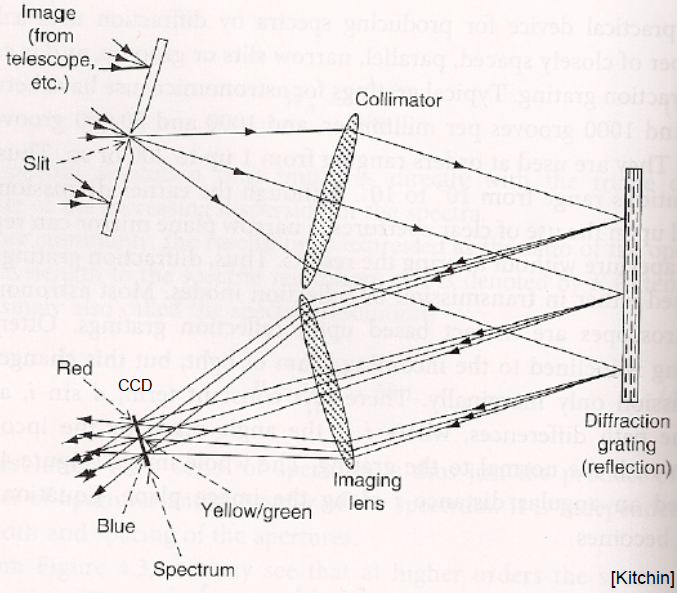
\includegraphics[width=0.5\textwidth]{Immagini/Capitolo3/Spettrografo_schema_reticolo_diff.PNG}
    \caption{Schema di uno spettrografo moderno a reticolo di diffrazione}
    \label{im:schema-spettroscopio-reticolo}
\end{figure}

Ora vale la pena analizzare i limiti di questo sistema, primo tra di essi le implicazioni che può avere sulla risoluzione spettrale, che va ora calcolata in base ad un pattern di diffrazione, e non più rifrattivo. Nella diffrazione, sappiamo che avere un limite nel distinguere due lunghezze d'onda equivale a dire di avere un limite sulla distinzione tra due angoli, per cui vale la pena interrogarsi su quale sia l'elemento ostruttivo nel percorso di diffrazione di Fraunhofer tale da imporre questa limitazione.

\begin{wrapfigure}{l}{0.35\textwidth}
    \centering
    \vspace{-5pt}
    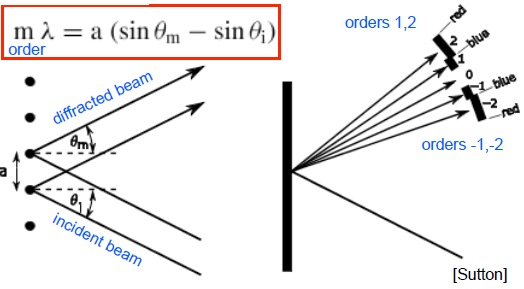
\includegraphics[width=0.34\textwidth]{Immagini/Capitolo3/Reticolo_diffrazione.PNG}
    \caption{Schema reticolo di diffrazione visto lateralmente}
    \label{im:schema-diff-reticolo}
    \vspace{-5pt}
\end{wrapfigure}

Nell'immagine \ref{im:schema-diff-reticolo}, che schematizza il reticolo di diffrazione, i solchi sono rappresentati dai punti, disposti simmetricamente a distanza $a$, detto passo del reticolo, e responsabili della diffrazione di Fraunhofer. Come si vede, il fascio incide parallelamente ad un angolo $\theta_i$ rispetto la normale al reticolo, per essere diffratto ad un angolo $\theta_m$ rispetto la normale, in direzione di dove viene appositamente messo il CCD. La distinzione tra due angoli differenti rimane sempre pari a $\lambda/d$, ma in questo caso $\lambda$ è dato dalle dimensioni fisiche del reticolo, le quali fanno da elemento ostruttivo dello spettrografo. L'equazione che correla angolo incidente e angolo diffratto ad una determinata lunghezza d'onda è la seguente, detta \textit{equazione del reticolo}:
\begin{equation}
    \label{eq:spett-reticolo}
    m\lambda = a \bigl(\sin\theta_m-\sin\theta_i \bigr)
\end{equation}
Essendo che è una condizione sui multipli interi, sarà verificata per vari valori di $m$ detti ordini, i quali presenteranno la stessa lunghezza d'onda ma ad intensità diverse per angoli di diffrazione diversi, come mostrato sempre nella \ref{im:schema-diff-reticolo}. Abbastanza spesso, anche nei telescopi di dimensioni maggiori, questi reticoli vengono combinati ad un elemento ottico, ad esempio con dei prismi, in modo da creare uno strumento in grado di disperdere la luce nella stessa direzione di incidenza, ma nuovamente per via della rifrazione. Il grande vantaggio introdotto da questa linearità sta nel fatto che si possa passare da un sistema spettrale nuovamente ad uno di imaging semplicemente togliendo questo reticolo, ad esempio sostituendolo con un filtro all'interno del telescopio. Torniamo ora ad una descrizione formale degli effetti che ha sulla dispersione e la risoluzione spettrali, differenziando la \ref{eq:spett-reticolo}, otteniamo:
\begin{equation*}
    md\lambda = a\cos\theta_m d\theta_m
\end{equation*}
In funzione dell'angolo di deviazione $\theta_m$, da cui possiamo ricavare la dispersione angolare come:
\begin{equation*}
    \frac{d\theta_m}{d\lambda} = \frac{m}{a\cos\theta_m}
\end{equation*}

\begin{wrapfigure}{r}{0.35\textwidth}
    \centering
    \vspace{-5pt}
    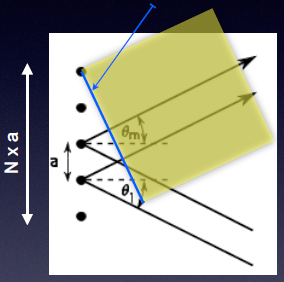
\includegraphics[width=0.34\textwidth]{Immagini/Capitolo3/Reticolo_fascio_diffratto.PNG}
    \caption*{Rappresentazione fascio diffratto}
    \vspace{-5pt}
\end{wrapfigure}

\noindent
Dove la dispersione è maggiore tanto maggiore sarà l'ordine a cui andiamo. Nel caso di $N$ solchi, sappiamo che le dimensioni lineari del reticolo devono essere $Na$, dove $a$ è il passo. qui risiede, come citato prima, una limitazione del reticolo, che come con i prismi, si ha che le sue dimensioni limitano la risoluzione disponbile: per fasci obliqui l'ampiezza di fascio diffratta sarà limitatamente pari a $Na\cos\theta_m$, poichè oltre queste dimensioni non c'è fisicamente nessun reticolo che possa sottoporre il fascio incidente a diffrazione e quindi riflessione. Si ricorda che la diffrazione è data esclusivamente da Fraunhofer, per cui non vi è il fattore $1.22$ e si mantiene il solo criterio di Rayleigh di $\lambda/d$, dove $d$ sono le nuove dimensioni del fascio, per cui il primo minimo sarà dato a:
\begin{equation*}
    \Delta\theta_m=\frac{\lambda}{Na\cos\theta_m}
\end{equation*}
Si ricorda che la risoluzione viene definita analogamente alla \ref{def:ris-ang} proprio in base alla distanza a cui si trova il primo minimo delle figure di diffrazione che si intendono risolvere, inserendo questo valore di $\Delta\theta$ nella versione differenziata della \ref{eq:spett-reticolo} otteniamo $\Delta\lambda=\lambda/m$, da cui ricaviamo la risoluzione spettrale come:
\begin{equation}
    \label{eq:spett-ris-spet-reticolo}
    R = \frac{\lambda}{\Delta\lambda} =
    mN =
    Na \frac{\sin\theta_m-\sin\theta_i}{\lambda}
\end{equation}
Dove si è adoperata la \ref{eq:spett-reticolo} nello sviluppo finale. Lo svantaggio principale di questi spettrografi a reticolo è che i vari ordini possono sovrapporsi, ad esempio il blu di primo ordine rischia di sovrapporsi al rosso di secondo ordine, andando a perdere range spettrale. Vedendo meglio questo concetto tra due ordini adiacenti:
\begin{equation*}
    a \Bigl( \sin\theta_m - \sin\theta_i \Bigr) =
    \Bigl( m+1 \Bigr) \lambda =
    m \Bigl( \lambda + \Delta\lambda \Bigr)
\end{equation*}
Da cui definiamo il \textit{range spettrale libero} $\Delta\lambda_{FSR}$, o \textit{intervallo spettrale libero}, come:
\begin{equation}
    \label{eq:spett-FSR}
    \Delta\lambda_{FSR} = \frac{\lambda}{m}
\end{equation}
Che è l'intervallo massimale di lunghezze d'onda per il quale non avviene copertura d'ordine, dal quale è ricavabile la distanza tra due massimi consecutivi corrispondenti alla stessa lunghezza d'onda.

Il motivo per cui, viceversa, si è sorpassato il modello a prisma sta nella capacità di poter raggiungere risoluzioni molto maggiori tramite l'adozione di reticoli, il primo sistema è infatti limitato dallo spessore del prisma (più è spesso maggiore la rifrazione), ma soprattutto dalla derivata dell'indice di rifrazione, il quale non cambia mai radicalmente con la lunghezza d'onda, infatti:
\begin{equation*}
    R_{prism}=t\frac{dn}{d\lambda}
\end{equation*}
Dove $t$ è lo spessore, la risoluzione dei sistemi a prisma è limitata dalla scarsa capacità dispersiva e difficilmente può superare il valore di mille, rendendoli poco adatti per studi particolarmente dettagliati. Un motivo aggiuntivo risiede nel fatto che i prismi hanno necessariamente efficienza ridotta anche nella trasmissione, essendo che il vetro assorbe parte del segnale entrante.

\section{Introduzione alla spettroscopia multi-oggetti}

Passando a risvolti maggiormente pratici, la spettroscopia può essere adoperata anche per una moltitudine di sorgenti in contemporanea. Per fare ciò basterà porre una piastra in alluminio (o di un qualsiasi materiale oscurante) di fronte al telescopio, intagliando delle fenditure rettangolari, tipicamente tramite laser per maggiore precisione, in corrispondenza delle fonti che si intendono isolare e studiare. La scelta delle fenditure rettangolari, piuttosto che quadrate, per studiare fonti essenzialmente sferiche, si giustifica con l'interesse che si ha nel introdurre anche il rumore di fondo spettrale del cielo, il quale verrà poi tolto in elaborazione tramite osservazioni indipendenti, esattamente come avviene per l'imaging.

\begin{wrapfigure}{l}{0.4\textwidth}
    \centering
    \vspace{-10pt}
    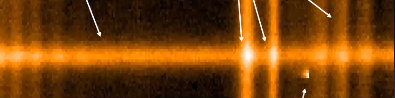
\includegraphics[width=0.39\textwidth]{Immagini/Capitolo3/Spettro_multi_concielo.PNG}
    \vspace{-5pt}
    \caption*{Spettro multi-oggetti compreso di cielo}
    \vspace{+8pt}

    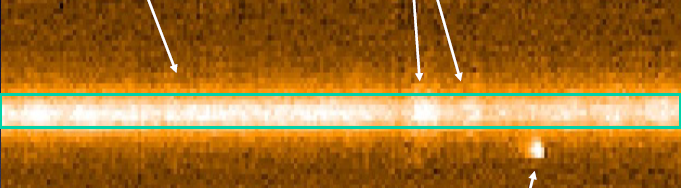
\includegraphics[width=0.39\textwidth]{Immagini/Capitolo3/Spettro_multi_senzacielo.PNG}
    \vspace{-5pt}
    \caption*{Spettro multi-oggetti sottratto di cielo}
    \vspace{-10pt}
\end{wrapfigure}

La tecnica è molto semplice: il cielo ha intensità luminosa maggiore, per cui è possibile isolarne lo spettro analizzando le zone limitrofe sufficientemente al di sopra e al di sotto dela direzione di dispersione orizzontale (in pixel), dove sono presenti solo le sue linee spettrali. Fatta questa analisi, è sufficiente rimuovere dallo spettro originario le linee trovate isolate nelle zone citate. Questa sottrazione, pur quanto utile nell'isolare lo spettro della sorgente, non può contribuire alla riduzione del rumore di fondo del cielo. Quest'ultimo dipende dalla radice del numero di fotoni entrante ed è imprescindibile, soprattutto nelle righe spettrali sulla linea di dispersione rimangono comunque residui della sottrazione del cielo. Per arrivare al plot finale, è necessaria una calibrazione del sistema, ossia associare ad ogni pixel del CCD (essendo che nella pratica si lavora in pixel) una specifica lunghezza d'onda. Questa calibrazione viene fatta tramite lampade di laboratorio il cui spettro è già noto, facendone arrivare la luce al cammino ottico del telescopio tramite fibra ottica, in tal modo è possibile calibrare il sistema su una scala completa di lunghezze d'onda tramite l'uso di più lampade. Fatto ciò, è possibile estrarre il flusso entrante nella fenditura (in conteggi) e mediarlo sulle corrispettive lunghezze d'onda associate ai pixel, ottenendo la \ref{im:spettro-plot-conteggi}.

\begin{figure}[htpb]
    \centering
    \begin{minipage}[c]{0.4\textwidth}
        \centering \setlength{\captionmargin}{0pt}
        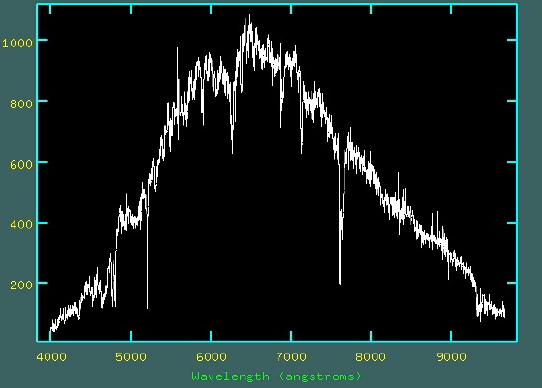
\includegraphics[width=0.97\textwidth]{Immagini/Capitolo3/Spettro_conteggi_plottato.PNG}
        \caption{Plot di uno spettro immediato (conteggi su Angstrom)}
        \label{im:spettro-plot-conteggi}
    \end{minipage}
    \hspace{5mm}
    \begin{minipage}[c]{0.4\textwidth}
        \centering \setlength{\captionmargin}{0pt}
        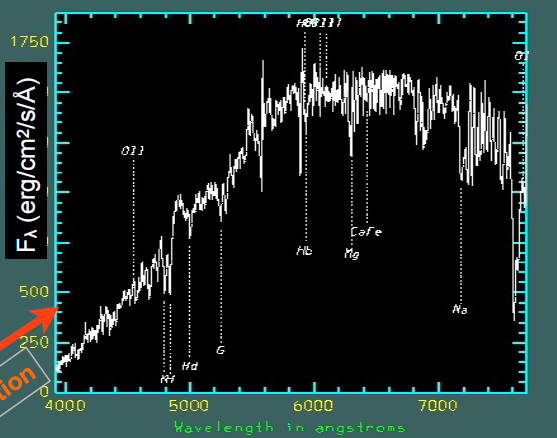
\includegraphics[width=0.9\textwidth]{Immagini/Capitolo3/Spettro_calibrato_flusso_plottato.PNG}
        \caption{Plot di uno spettro calibrato in flusso (flusso su Angstrom)}
        \label{im:spettro-plot-calibrato-flusso}
    \end{minipage}
\end{figure}

Chiaramente, nel valutare questo grafico va tenuto in considerazione che esso non corrisponda direttamente allo spettro della fonte ma al prodotto di quest'ultimo per la funzione di risposta spettrale, data dall'efficienza dello spettrografo e quindi dalla struttura del reticolo adottato (in generale dall'elemento dispersore). Per passare da conteggi a flusso, è necessaria un'ultima calibrazione, detta \textit{calibrazione in flusso}, tramite l'osservazione di stelle "standard" il cui flusso spettrale è già noto in modo da poter far corrispondere il flusso in conteggi in un effettivo flusso spettrale in unità fisiche, ottenendo la \ref{im:spettro-plot-calibrato-flusso}. Si notano nel plot alcune righe particolarmente lunghe, le quali corrispondono ai residui della sottrazione del cielo, la quale non risulta mai perfetta e lascia comunque queste linee di rumore.

Questa tecnica va applicata ad ogni sorgente isolata tramite una corrispodente fenditura, adoperato lo stesso elemento dispersore. Un'altra utilità del rumore di fondo del cielo, sempre il medesimo in one ristrette di cielo, è che aiuta nella misurazione del redshift. Di fatti, se due sorgenti isolate vengono mandate allo spettrografo, ma esse si trovano ad entrare ad ascisse diverse rispetto la fenditura, allora necessariamente per motivi geometrici ci sarà uno shift aggiuntivo nelle lungheze d'onda, nonostante la dispersione sia la medesima avendo adoperato lo stesso reticolo. Grazie al confronto delle linee di cielo tra due spettri diversi, questo shift "geometrico" è isolabile rispetto al redshift. Questa in sunto è la spettroscopia a multi-oggetti, molto adoperata nella mappatura delle galassie nell'universo grazie alla misurazione del redshift.

\begin{wrapfigure}{r}{0.41\textwidth}
    \centering
    \vspace{-10pt}
    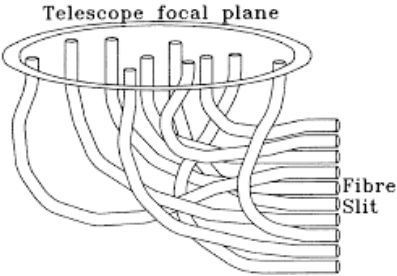
\includegraphics[width=0.4\textwidth]{Immagini/Capitolo3/Telescopio_schema_fibra.PNG}
    \caption*{Schema telescopio a fibra ottica}
    \vspace{-5pt}
\end{wrapfigure}

Negli ultimi anni, anche grazie alla sempre maggiore robotizzazione, si è superato questo modello a copertura tramite alluminio del sistema ottico, poichè richiedente molto tempo per la preparazione e un notevole dispendio in materiali. Ora il sistema più utilizzato sfrutta una serie di \textit{fibre ottiche} direttamente allocate sul piano focale del telescopio, le quali possono essere traslate e isolano perfettamente la zona del piano interessata. Queste fibre sono tra di loro isolate, permettendo così di poter adoperare spettrografi diversi per sorgenti diverse, a seconda del tipo di indagine che si vuole svolgere (più o meno dispersivi, a maggiore o minore risoluzione). Il principale limite risiede nel fatto che ogni fibra ottica ha la sua efficienza e che chiaramente essendo dei tubi non possano essere affiancate tra di loro senza ottenere un'immagine finale a griglia, per cui non risultano adatti qualora si voglia campionare un'intera galassia parte per parte.

Un'alternativa che si è tornata ad usare sono i \textit{telescopi slitless}, i quali disperdono direttamente l'intera immagine catturata e con essa tutte le sorgenti che ne fanno parte. Questi telescopi risultano particolarmente adatti per esperimenti spaziali, ad esempio è stato adoperato sul telescopio GAIA per le misure di parallasse e di effetto Doppler tramite lo spettrografo, con il quale sono state classificate un decimo delle stelle della galassia. Il principale vantaggio è quello di disperdere contemporaneamente diverse sorgenti, ma al tempo stesso questo comporta che, presa l'ascissa come direzione di dispersione, due sorgenti poste sulla stessa ordinata avranno spettri sovrapposti. Il secondo grande svantaggio è avere un grande contributo del rumore del cielo, il quale non essendo più isolato in una frazione della fenditura viene disperso al pari delle sorgenti, dando un disturbo sull'ordine delle migliaia di volte maggiore rispetto la tecnica vista in precedenza, motivo per cui questa tecnica è inadoperabile da terra.

\begin{figure}[htpb]
    \centering
    \begin{minipage}[c]{0.4\textwidth}
        \centering \setlength{\captionmargin}{0pt}
        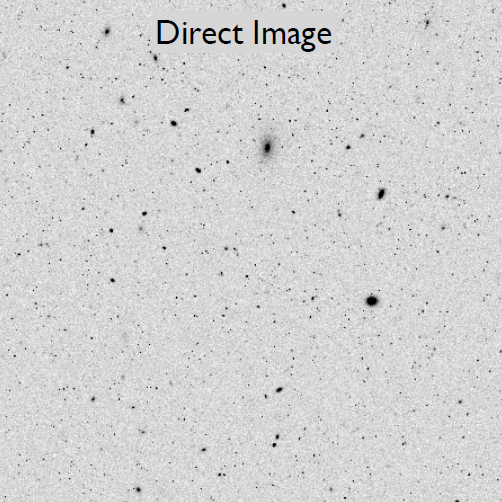
\includegraphics[width=0.9\textwidth]{Immagini/Capitolo3/Telescopio_slitless_immagine.png}
        \caption*{Immagine diretta}
    \end{minipage}
    \hspace{5mm}
    \begin{minipage}[c]{0.4\textwidth}
        \centering \setlength{\captionmargin}{0pt}
        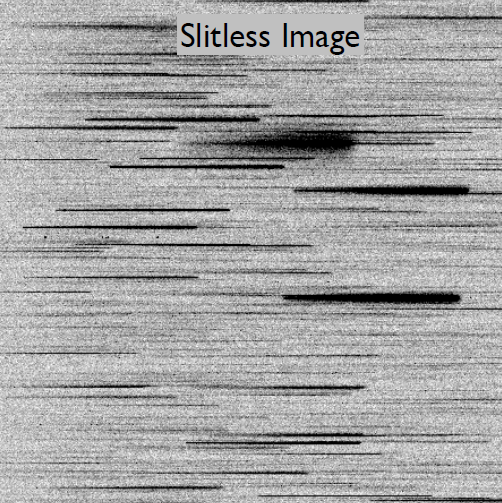
\includegraphics[width=0.9\textwidth]{Immagini/Capitolo3/Telescopio_slitless_spettro.png}
        \caption*{Immagine spettro slitless}
    \end{minipage}
    \caption{Spettroscopia slitless}
    \label{im:spettroscopia-slitless}
\end{figure}

Questo tipo di spettrografi verrà adoperato anche nel prossimo satellite Euclid, in partenza nel 2023, dedicato alla cosmologia e disegnato per mappare in tre dimensioni la distribuzione delle galassie più lontane tramite misurazioni di redshift di migliaia e migliaia di spettri, in ricerca di evidenze della materia oscura. Una versione più elaborata di questa tecnica per l'analisi tridimensionale sta negli \textit{slicing mirrors}, specchi sagomati a più livelli ricavati dal pieno, ognuno ad inclinazione diversa, i quali riflettono l'immagine tagliandola a fette(slicing) e mandandola ad una serie di specchi secondari con i corrispettivi dispersori. In tal modo è possibile spezzare immagini molto grandi, ad esempio di galassie, in varie parti ed in diverse direzioni, ottenendo uno spettro tridimensionale di esse.

\chapter{Telescopi a raggi X}

\section{Introduzione ai telescopi a raggi X}

Un contributo recente e fondamentale all'evoluzione dell'astrofisica si trova negli anni '60 dello scorso secolo, con prime realizzazioni negli anni '70, e riguarda l'approdaggio della banda X allo studio dei corpi celesti. Il motivo per cui si aggiunse così in ritardo questa banda rispetto a quella dell'ottico e dell'infrarosso viste fino ad ora, sta nella difficoltà che energie e frequenze così implicano nel riuscire a fuocheggiare i raggi entranti. Negli anni '60 i raggi X erano rilevabili prevalentemente da rilevatori Geiger e similari, in più senza possibilità di fuocheggiarli in un'area ridotta si avrebbe sia un rapporto segnale-rumore grandissimo, sia una forte limitazione di osservazione a quelle che sono le dimensioni dell'area collettrice del detector. Viste queste notevoli problematiche, in quegli anni Riccardo Giacconi e Bruno Rossi iniziarono a cercare un modo per riflettere e fuocheggiare questi raggi, sfruttando un principio di riflessione già noto all'epoca. I raggi X trovano nei materiali ad elevato numero atomico Z (i metalli) un mezzo otticamente meno denso, i cui indici di rifrazione rispetto ai fotoni in quella banda sono di poco minori a uno. Ricordando la legge di Snell:
\begin{equation}
    \frac{\sin\theta_i}{\sin\theta_r}=\frac{1}{n_{X-ray}}
\end{equation}
Ne consegue che l'angolo di riflessione rispetto al piano di riflessione di questi materiali è leggermente maggiore di quello incidente, per cui è possibile fuocheggiare raggi X tramite sistemi poco curvi posti in direzione radente rispetto quella di incidenza. In questo caso il fenomeno di riflessione e rifrazione è simile a quanto avviene nell'ottico, ci sarà un determinato valore detto \textit{angolo critico} per cui i raggi riflessi sono paralleli al piano del materiale (o meglio al piano che separa i due mezzi a densità ottica diversa). Al di sotto di questo valore non vi è una separazione del fascio in riflessione o rifrazione ma si osserva una riflessione totale. Si ricorda la definizione di questo angolo critico come:
\begin{equation*}
    \cos\theta_c = n_{X-ray} =
    1-\delta \quad \longrightarrow \quad
    \theta_c \simeq \sqrt{2\delta}
\end{equation*}
Dove si è introdotto il parametro $\delta$ per definire lo scarto tra l'indice di rifrazione del mezzo nella banda X e l'unità per pure ragioni di comodità, essendo che tutti gli indici che vengono trattati hanno uno scarto negativo piccolissimo rispetto all'unità.


\end{document}